%%%%%%%%%%%%%%%%%%%%%%%%%%%%%%%%%%%%%%%%%
% Journal Article
% LaTeX Template
% Version 1.4 (15/5/16)
%
% This template has been downloaded from:
% http://www.LaTeXTemplates.com
%
% Original author:
% Frits Wenneker (http://www.howtotex.com) with extensive modifications by
% Vel (vel@LaTeXTemplates.com)
%
% License:
% CC BY-NC-SA 3.0 (http://creativecommons.org/licenses/by-nc-sa/3.0/)
%
%%%%%%%%%%%%%%%%%%%%%%%%%%%%%%%%%%%%%%%%%

%----------------------------------------------------------------------------------------
%	PACKAGES AND OTHER DOCUMENT CONFIGURATIONS
%----------------------------------------------------------------------------------------

\documentclass[twoside,twocolumn]{article}

\usepackage{graphicx}
\usepackage{amsmath}

\usepackage[sc]{mathpazo} % Use the Palatino font
\usepackage[T1]{fontenc} % Use 8-bit encoding that has 256 glyphs
\linespread{1.05} % Line spacing - Palatino needs more space between lines
\usepackage{microtype} % Slightly tweak font spacing for aesthetics

\usepackage[english]{babel} % Language hyphenation and typographical rules

\usepackage[hmarginratio=1:1,top=32mm,columnsep=20pt]{geometry} % Document margins
\usepackage[hang, small,labelfont=bf,up,textfont=it,up]{caption} % Custom captions under/above floats in tables or figures
\usepackage{booktabs} % Horizontal rules in tables

\usepackage{lettrine} % The lettrine is the first enlarged letter at the beginning of the text

\usepackage{enumitem} % Customized lists
\setlist[itemize]{noitemsep} % Make itemize lists more compact

\usepackage{abstract} % Allows abstract customization
\renewcommand{\abstractnamefont}{\normalfont\bfseries} % Set the "Abstract" text to bold
\renewcommand{\abstracttextfont}{\normalfont\small\itshape} % Set the abstract itself to small italic text

\usepackage{titlesec} % Allows customization of titles
\renewcommand\thesection{\Roman{section}} % Roman numerals for the sections
\renewcommand\thesubsection{\roman{subsection}} % roman numerals for subsections
\titleformat{\section}[block]{\large\scshape\centering}{\thesection.}{1em}{} % Change the look of the section titles
\titleformat{\subsection}[block]{\large}{\thesubsection.}{1em}{} % Change the look of the section titles

\usepackage{fancyhdr} % Headers and footers
\pagestyle{fancy} % All pages have headers and footers

% \fancyfoot[RO,LE]{\thepage} % Custom footer text

\usepackage{titling} % Customizing the title section

\usepackage{hyperref} % For hyperlinks in the PDF

%----------------------------------------------------------------------------------------
%	TITLE SECTION
%----------------------------------------------------------------------------------------



\setlength{\droptitle}{-4\baselineskip} % Move the title up

\pretitle{\begin{center}\Huge\bfseries} % Article title formatting
\posttitle{\end{center}} % Article title closing formatting
\title{\href{https://github.com/vsalova/lane_lines}{EEC 193 Autonomous Car Senior Design Report}} % Article title
\author{%
\textsc{Calvin Cramer, Daniel Loran, Victoria Salova} \\ % Your name
\normalsize University of California, Davis \\ % Your institution
}
\date{\today} % Leave empty to omit a date

%----------------------------------------------------------------------------------------

\begin{document}

% Print the title
\maketitle

%----------------------------------------------------------------------------------------
%	ARTICLE CONTENTS
%----------------------------------------------------------------------------------------

\section{Summary}

\par Lane line detection is one of the most fundamental systems of autonomous driving. Detecting lane lines serves as a basis module, on top of which path planning and other parts may be built. Knowing this, the lane line detection module must be robust, reliable, and accurate in order for these other systems to work. Even for non-self driving cars, lane line detection is the main component behind lane departure warning systems, and automatic steering in highway environments.
\par For this project, the first part was to combine two different versions of the lane line detection lab from Winter quarter and to find the speed and accuracy for use as a benchmark. The next goal was to find replacements for window search, such as using clustering algorithms, and also replacing one-dimensional window search with a two-dimensional search. The next part was to try and implement various deep learning models and see how they compare to classical computer vision approach.

%------------------------------------------------

\section{Data Sets}
\subsection{Formatting CULane annotations - Calvin}
\par The CULane dataset is a dataset of Beijing roads. The annotations included are for background, left-left lane, left lane, right lane, and right-right lane. Strangely, the annotations in the dataset are fixed width lanes from the car's perspective. An example of this can be seen in figure \ref{fig:og}.

\begin{figure}
  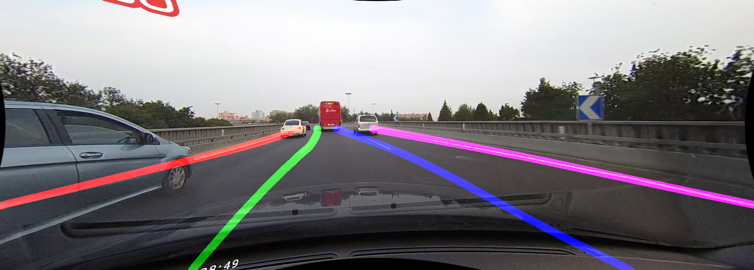
\includegraphics[width=\linewidth]{calvin3.png}
  \caption{Original CULane labels.}
  \label{fig:og}
\end{figure}

\par From the car's perspective lane lines start out thickest at the bottom and get thinner as the lane is further out. We decided to change these annotations to overlap the actual lane precisely, with tapering. The reformatted annotation for figure \ref{fig:og} is given in figure \ref{fig:updated}.

\begin{figure}
  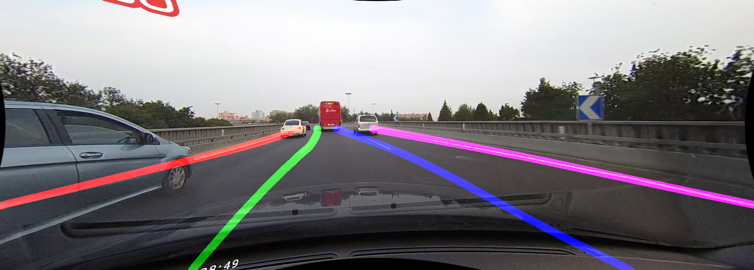
\includegraphics[width=\linewidth]{calvin3.png}
  \caption{Updated CULane labels.}
  \label{fig:updated}
\end{figure}

\par The purpose of reformatting the annotations like this is to train our deep learning models to detect just the lane, and not the surrounding space. An argument can be made to detect more of the lane in the distance, in order to give the model more of a chance to learn to detect the lane in the distance. Future work needs to be done to determine the validity of this, but post processing through dilation may help mitigate a small number of pixels for lanes in the distance.
\par Additional work can be done to round the end of the annotations, have a more reasonable drawing thickness for the left-left and right-right lanes, to determine the start and stop of each lane, and some tuning on the polynomial regression part of this reformatting procedure. Additionally, it may be useful to undistort the image into a top-down view, which may increase the accuracy of the output annotations.

\subsection{Scripts for CULane converstion - Calvin}
\par The original annotations in CULane are given as one channel images with the values 0 for background, 1, 2, 3, and 4 for the left-left, left, right, and right-right lanes respectively. For the different deep learning models we used, all of them require the annotations to be in different formats, so we made scripts to convert the CULane annotations into these formats. An example of this is the the ICNet model requires RGB images, so the images were converted to RGB. Also, in order to actually see the annotations we mapped the 1, 2, 3, 4 values to high values, because if you open up the original annotations as a picture they look completely black.
\par Another script we wrote was to calculate the average RGB value for the whole CULane dataset train and test images. ICNet needed this average value in order to train properly.
\par Another script we wrote converted a directory of images into an avi video. The use of this script was to combine the output images from LaneNet into a video, since we didn't have a script that could automatically run LaneNet and convert the output images into a video, rather than just saving all of the images separately.
\par We also had a script to visualize the difference between the original CULane annotations and the reformatted annotations.
\par Another little script was to copy specific files (stored as paths in a file) to one location. The purpose of this was to gather specific test images from CULane that are representative of different driving conditions. CULane details many different driving scenarios, such as day, night, rain, no lanes, pedestrian, arrows, et. cetera. We gathered all of the images into one place (data/CULane/ folder in repo) in order to test out methods in these different scenarios.


%------------------------------------------------

\section{Classical Computer Vision Approach}

\subsection{Benchmark for Lab 1 - Calvin}
\par In order to explore different methods that work on top of the lab 1 pipeline, it was necessary to determine the most expensive parts of the pipeline. This allowed us to explore replacements for certain parts in the pipeline with the knowledge of how it would affect the running time of the pipeline. The benchmark measures the total times and frames per second for image distortion/warping operations, histogram, window search, waypoint generation, and a few others.

\begin{figure}
  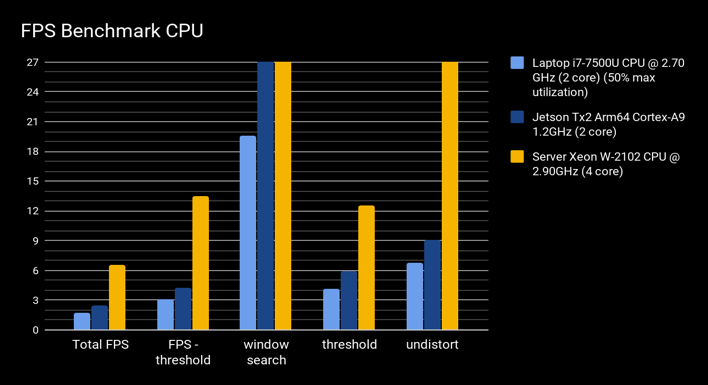
\includegraphics[width=\linewidth]{calvin1.png}
  \caption{FPS Benchmark CPU}
  \label{fig:cpu}
\end{figure}

\begin{figure}
  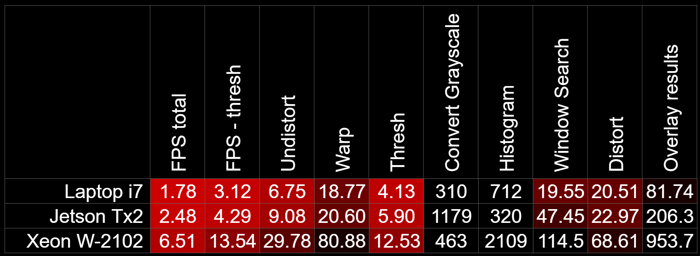
\includegraphics[width=\linewidth]{calvin2.png}
  \caption{Benchmark results}
  \label{fig:benchmark}
\end{figure}

\par The benchmark was ran on three computers: Calvin's laptop, the Kronos server, and a Jetson TX2. The program ran completely on CPU, which is important to keep in mind when interpreting the results. The CPUs for these machines were an Intel i7-7500U (4 cores) capped at 50\% max utilization, Jetson Tx2 Arm64 Cortex-A9 1.2GHz (2 cores), and an Intel Xeon W-2102 CPU @ 2.90GHz (4 cores) respectively.

\par Figure \ref{fig:cpu} and figure \ref{fig:benchmark} show the results of the benchmark. The results of the benchmark show that common image manipulations are the bulk of the runtime. The main lane localization part (histogram, window search, polynomial regression) took a trivial amount of time. From this it is worthwhile to explore running the image manipulation parts of the pipeline on GPU, which is the type of operations GPUs are built for.


\subsection{Calculation of Radius of curvature and lane offset - Calvin}
\par From the detected lane lines from the lab 1 pipeline (and any model where a polynomial of the lane is detected) we can calculate some important information that is vital for safety warning systems. The two pieces of information we calculated were radius of curvature \ref{eq:ROC} and lane offset \ref{eq:offset}. The radius of curvature shows how straight or curved the detected lane is. A safety system may take this information into account, and can predict that if the driver turns to rapidly, that they may go past the lane. Lane offset explains itself nicely: it is the offset of the vehicle from the center of the lane. This information is a useful bit of information for lane departure warning systems. If we can detect that the lane is underneath the left or right wheels of the vehicle, and the driver is not changing lanes, then the driver may not be paying attention and drifting outside of the lane. Another use of this information is for a lane following system, where the system can try to minimize the offset from the center of the lane in order to automatically follow the center of the lane.
\par The calculation for the radius of curvature and the lane offset were fairly simple, all that was needed for the radius of curvature was to take the function for each lane and get the first \ref{eq:derivative} and second derivative \ref{eq:derivative2}, and use a special formula. Note that the lanes are a function of y instead of x. The calculation for the offset of the vehicle in the lane is even simpler, using the assumption that the camera is in the very center of the vehicle. If this is the case, then the offset is just the pixel difference between the center of the detected lanes and the center of the video frame, multiplied by the radio between meters and pixels in the x direction. If the camera is not in the exact center of the vehicle, then this calculation can be calibrated by adding an offset to the "center-line" of the video frame.

\begin{subequations}
\begin{align}
f(x) &= ax^2 + bx + c \\
f'(x) &= 2ax + b \label{eq:derivative} \\
f''(x) &= 2a \label{eq:derivative2}
\end{align}
\end{subequations}

\begin{align} \label{eq:ROC}
RoC &= \frac{[1 + f'(x)^2]^\frac{3}{2}}{f''(x)}
\end{align}

\begin{subequations}
\begin{align}
center &= \frac{x_{l} + x_{r}}{2} \\
x_{l} &= lane_{l}(h_{window} - 1) \\
x_{r} &= lane_{r}(h_{windiw} - 1) \\
offset &= \frac{W_{window}}{2} - center \label{eq:offset}
\end{align}
\end{subequations}

\subsection{Replacements for window search - Daniel}

\par The traditional computer vision approach to lane line detection is considered to simpler and less resource intensive than a neural network based approach. At the beginning of this project, a 5 stage modular pipeline (undistort image, RoI, thresholding, recursive window search, polyfit) was initially considered for modification. The recursive window search module was identified as an algorithm that could be replaced by a faster module due to its recursive nature.

\begin{figure}
  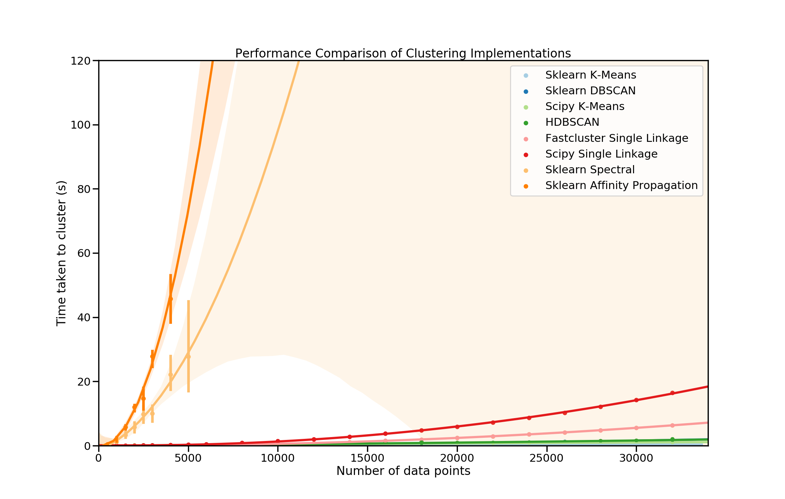
\includegraphics[width=\linewidth]{daniel1.png}
  \caption{Benchmark: data points vs time taken for different clustering algorithms}
  \label{fig:d1}
\end{figure}

\par Since clustering can be ran on all points in an image or bitmap, the motivation was to replace the recursive window search algorithm with a series of clustering algorithms, both to reduce noise and find lane lines in a non-recursive fashion. In order to do this, multiple clustering algorithms needed to be tested. It can be seen in figure \ref{fig:d1} the results of a benchmark test done on bitmaps of similar size and density to the ones that the previous thresholding step would produce. The sklearn k-means clustering algorithm stood out as a very fast clustering algorithm, although using kmeans would mean that the number of lanes must be known beforehand. HDBscan tests as a fairly slow algorithm but comes with the added functionality of identifying and filtering out points the algorithm deems noise.

\begin{figure}
  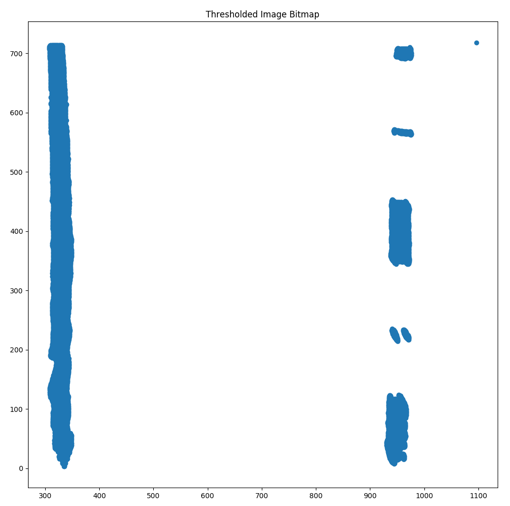
\includegraphics[width=\linewidth]{daniel2.png}
  \caption{Input bitmap to clustering module}
  \label{fig:d2}
\end{figure}

\par The proposed clustering module has two steps. Initially, a bitmap is taken in from the thresholding module (figure \ref{fig:d2}). HDBscan is applied first to the bitmap to group points into initial clusters, while also removing noise (figure \ref{fig:d3}). Then, for each cluster a centroid point and a top y-value point are selected. After the centroid and y-value pairs are identified, they are clustered into left and right lanes using k-means clustering. After the k-means clustering, linear regression is run to estimate where the lines are (figure \ref{fig:d4}).

\begin{figure}
  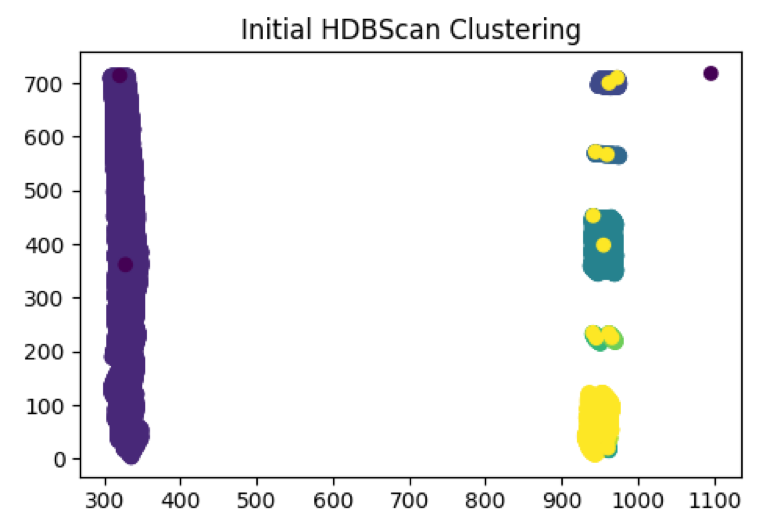
\includegraphics[width=\linewidth]{daniel3.png}
  \caption{Initial HDBscan clustering}
  \label{fig:d3}
\end{figure}

\begin{figure}
  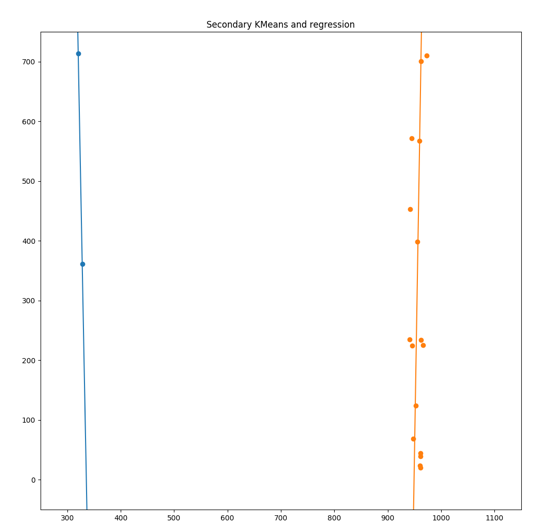
\includegraphics[width=\linewidth]{daniel4.png}
  \caption{Post linear regression}
  \label{fig:d4}
\end{figure}

\par This clustering module ends up running at approximately 1.4 FPS, with limitations on what sort of noise it can handle in input images. Additionally, the clustering module is not able to handle curved lane lines, since it assumes a straight line is drawn between the centroid and high y-value pairing. HDBscan is most responsible for the low speed of this module. Changing parameters such as min\_cluster\_size and min\_samples can result in a speed up but run the risk of decreasing accuracy. Future work on this module can be done in three areas - increasing resilience to noise, adding curve lane line prediction functionality, and increasing speed. Solving one of these problems might affect the solution of another problem; since HDBscan is used in part to remove noise, a new solution to noise in the bitmap might eliminate the need for HDBscan altogether, which might yield a speed increase.


\subsection{Initial foray into 2D Window search - Calvin}
\par One additional avenue to improve upon the original pipeline is to make the window search algorithm more robust to highly curved lanes. In order to do this, we needed to overcome the implicit limitation of the one-dimensional window search, which is that it can only detect lanes at most at a 45 degree angle. For most driving circumstances this limitation is not an issue, but there are situations such at roundabouts or parking lots where it is necessary to detect sharp turns.
\par In order to turn the one-dimensional window search into two-dimensions, we need turn the displacement of the window from a one dimensional update in the y dimension into a displacement in any direction. Making the displacement into a vector brings a lot of uncertainty about when the algorithm will terminate. It is impossible to know the number of steps the algorithm will take beforehand, as opposed to one-dimensional window search which always terminates in a specified number of steps (which determines the window height).
\par We placed the following stopping conditions on the search:
\begin{itemize}
\item Terminate if the window reaches close to the left, top, or right of the image
\item Terminate if the number of windows is greater than some specified amount
\end{itemize}
Another possible stopping conditions is to only allow the search to go "up" once, since we make the assumption that the lane lines start from the bottom of the image and that they curve nicely, generally in the upwards direction. It would not make much sense to see a lane line go up, and the back towards the car.
\par With these assumptions, we added a maximum angle change parameter, so that the search would smooth out, and not make drastic jumps in the angle of the displacement. Future work needs to be done to exploit this more, in the sense of using a PID controller to smooth the angle of displacement, and to give the search a general path or curve to follow when the current window doesn't have and lane line pixels, and must make a guess of where to go next based upon previous information. The guess we make on previous information now is simply to take the last displacement seen and continue in that direction. The PID controller may also help with oscillations that arise in this method. Since we are taking a step in the direction of where we see the lane line pixels, if we start a little bit off-center from the lane line at the bottom of the image then the algorithm may follow the lane but oscillate from the left of the lane to the right of the lane. In order to mitigate this we centered the first window with the nearby pixels, rather than starting from the histogram peak which may not be a good starting point for the lane.
\par Additional future work needs to be done to ensure that lane line points that are detects as "in the lane" are not double counted. This problem arises in 2D window search because the displacement radius is a tunable parameter, which may lead to successive windows overlapping. This problem is non-existent in one-dimensional window search because the displacement of the windows makes it impossible for the windows to overlap. Additional future work includes tuning the input parameters for this method. The parameters include maximum angle change, displacement radius, window width, window height, maximum number of windows, and the minimum number of pixels needed to consider a window signal (not noise).

\subsection{Comparison between 1D and 2D window search - Calvin}
\par The goal of the two-dimensional window search is to perform better on tight curves than the one-dimensional window search. This needs to be tested to see the difference between the two methods. In particular, the difference should be tested in various video scenarios.


\subsection{Experimentation with vector field (see hough branch) - Calvin}
\begin{figure}
  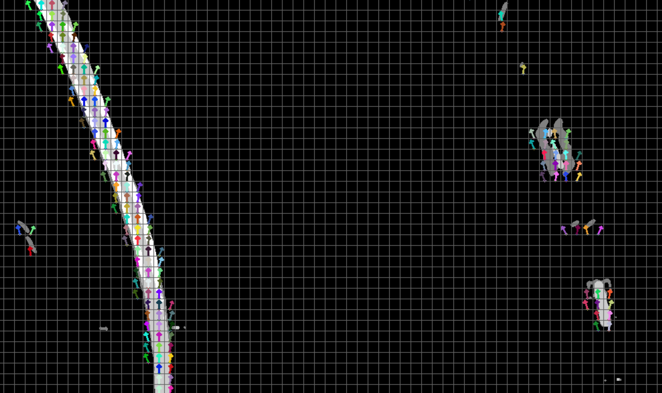
\includegraphics[width=\linewidth]{calvin5.png}
  \caption{Vectors}
  \label{fig:vectors}
\end{figure}

\par We originally started another lane line detection pipeline by converting the thresholded bitmap image to a vector field. The process of this was to split the image into a grid, and for each cell make a vector between the bottom-center of the cell and the average point of the top-most n rows of the cell. Although this part was not used in any pipeline, it's idea is fairly similar to the two-dimensional window search, and further work needs to be done to incorporate this in a complete pipeline or to incorporate the vector field in a two-dimensional search. An example of the vector field is included in figure \ref{fig:vectors}.


%------------------------------------------------

\section{Deep Learning Approaches}

\subsection{SCNN - Victoria}
\par The first neural net we looked at was Spatial CNN. It is a generalization of deep convolutional to a spatial level and it outperforms recurrent neural nets, Markov random fields, and conditional Random field, by both speed and accuracy.  SCNN views rows and columns of feature maps as layers and applies convolution and nonlinear activation sequentially, forming a deep neural network. The advantage of SCNN over other lane line detection methods is the fact that sequential message pass scheme is more computationally efficient than other RNN or Markov Random Field approaches - it gets rid of computational redundancy that other models have. It utilizes sequential propagation scheme instead of each node receiving messages from all others. So information goes  from right to left and top to bottom, so 4 directions, which results in the same amount of information to be passed, but with less computation. SCNN can also be incorporated into any part of CNN, rather than just the output. The ablation study that was done on SCNN shows that every part of this network is important  and not redundant. SCNN distinguishes each lane line as its own class, creates a probability map for each, which give prediction on the existence of the lane line markings. After that, these predictions are connected by cubic splines to create the final predictions of the lane lines. SCNN was compared to ReNet, MRFNet, DenseCRF, and the very deep residual network. Out of all the methods listed, SCNN performed significantly better, showing the best results.

\par In order to get this model running, we spent a significant amount of time setting up a proper docker container that would allow us to use the GPU for training. We also edited parts of the training script, updating the outdated tensorflow functions as well as editing the scripts to train on CULane dataset. Unfortunately, we decided not to proceed with this model as we realized we did not have the hardware to train this model. The last error that we ran into was GPU running out of memory. The attempts to decrease the batch size and other configuration settings to decrease the memory used turned out unsuccessful and we decided not to proceed with this model.


\subsection{LaneNet post-processing - Calvin}
\par The purpose of post-processing the output of LaneNet to fit polynomial lines to the lane predictions of LaneNet. Additionally, the output of LaneNet would swap the annotation class of the lane lines frequently, so an additional task here is to give each lane a consistent class, according to their location on the image.
\par Post-processing is done by taking each unique class in the input image, and doing polynomial regression to draw a smooth lane. The output of the post-processing were not good enough at this point, and can be improved by undistorting the image, and doing polynomial regression with for a lower order polynomial, and possibly dilating the input image to have more pixels to do regression on. Additionally, the RoC and lane-offset parts can be included here.
\par The way that we gave lane lines a consistent class was so sort the centers of the lane lines according to the angle from the center top of the frame. This gave fairly good results, but the classes were not 100 percent consistent in our output video. The reason for this is that sometimes a lane may not be present, and the algorithm assumes that all of the lanes will be present. A simple check to see if each lane line class is present or not may solve this problem.



\subsection{ICNet - Victoria}

\par The next deep learning approach we looked at was ICNet. The reason for this choice was that ICNet is one of the only semantic segmentation models that can run close to real time. The way ICNet works is that it downsamples a large input image by 1/2 and then by 1/4. The smallest image is ran through a heavy CNN and the two smaller ones are ran through a light CNN. A cascade feature fusion unit is then used to combine the results of the images to refine the segmentation in the higher resolution image. The reason ICNet is able to run so quickly while maintaining accuracy is because a heavy CNN is ran only on the smallest image, taking significantly less time than if it were run on the original image, so the run time is shortened significantly.
\par Just as with SCNN, the set up took a significant amount of time. The biggest challenge was finding the correct docker image that would allow us to train our model on the GPU. The model for the code that we used and its documentation were outdated, so we had to adapt the code to run on our systems. Most of the initial updates were debugging and replacing the outdated tensorflow functions.

\begin{figure}
  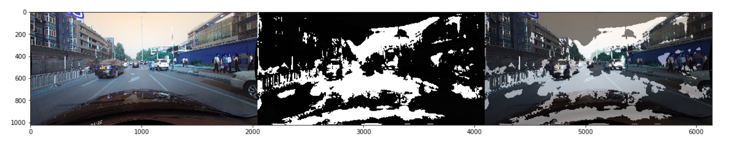
\includegraphics[width=\linewidth]{1.png}
  \caption{First ICNet training resuts.}
  \label{fig:first}
\end{figure}

\begin{figure}
  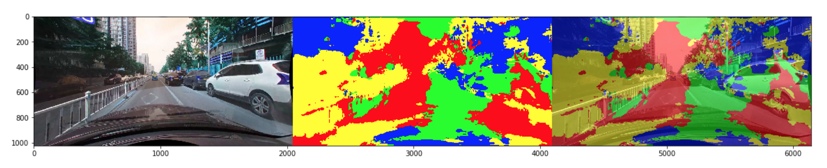
\includegraphics[width=\linewidth]{2.png}
  \caption{Smallest image weighted the most.}
  \label{fig:weights1}
\end{figure}

\begin{figure}
  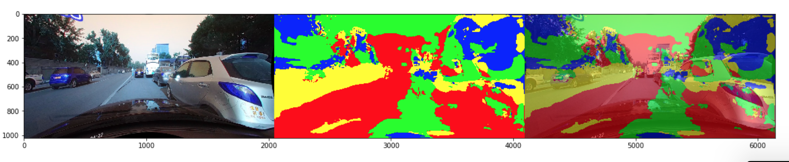
\includegraphics[width=\linewidth]{3.png}
  \caption{Image downsized by 1/2 is weighted the most.}
  \label{fig:weights2}
\end{figure}

\begin{figure}
  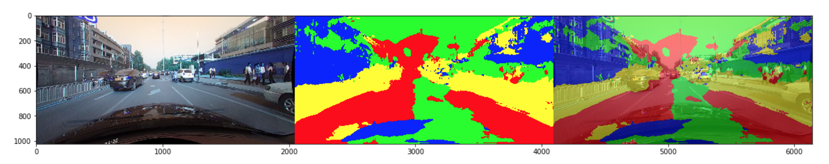
\includegraphics[width=\linewidth]{4.png}
  \caption{The original image is weighted the most.}
  \label{fig:weights3}
\end{figure}

\par Since ICNet was designed as a semantic segmentation model for scene understanding and trained on Cityscapes dataset, we couldn't use the pretrained weights and had to train the model from scratch. On average, it took about 14 hours to run the 60000 steps to train the model. The first run did not produce any results and just classified the entire image as background. Since we are trying to convert this model to predict lane line (which is a semantic segmentation subproblem) and are using the CULane dataset instead of Cityscapes, we had to refactor some parts of the training and evaluating scripts. First step was to relabel the CULane labeled images to have RGB labels, instead of grayscale. Another step was also to change the labels in the model. The CULane dataset consists of 5 labels -- 4 lane lines and background. Each lane line from left to right has its own class and there could be up to 4 lane lines labeled in each image (figure \ref{fig:labels1}). The labels also go through the obstacles in the image, such as cars, and are drawn over that, even if the actual lane line is not present in the image.  After that, we trained the model for the first time using the arbitrary parameters that were used in the original ICNet implementation. After the first training, the evaluation showed 19\% IoU and the result in figure \ref{fig:first} shows only one of the labels, but it is very clear that the label is all over the place.


\begin{figure}
  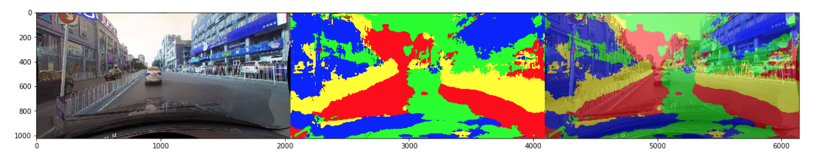
\includegraphics[width=\linewidth]{5.png}
  \caption{The image with the best weights.}
  \label{fig:best}
\end{figure}

\par For the next step, we tried adjusting weights differently for each of the images, getting slightly better results, but still needing more tuning, figures \ref{fig:weights1}, \ref{fig:weights2}, \ref{fig:weights3}.

\begin{figure}
  
\includegraphics[width=\linewidth]{6.png}
  \caption{The image with less occlusions.}
  \label{fig:occlusions}
\end{figure}

\par The figures \ref{fig:best} and \ref{fig:occlusions} use the same weights, but figure \ref{fig:occlusions} has a less occluded environment. The IoU for this iteration was about 86\%. In the figures, the label colors do not match exactly. But it is obvious in the last image, that the labels are encompassing the entire lane lines, and the surrounding areas as well, which is a problem throughout all the iterations above --- the entire image is labeled using the labels, ignoring the background completely. As we looked through the code, there was an ignore label in configurations. Eliminating that variable, however, did not change the results, neither did adding a dummy label and setting the ignore label to this dummy label. To fix this problem, we once again relabeled the dataset, figure \ref{fig:labels2}, but this time we decided to do just a binary classification: lane line and not a lane line. This was the last test we could run before the deadline, and the results were unsatisfactory, where the entire image was labeled as one class, figure \ref{fig:badbad}.

\begin{figure}
  
\includegraphics[width=\linewidth]{7.png}
  \caption{Original Labels}
  \label{fig:labels1}
\end{figure}

\begin{figure}
  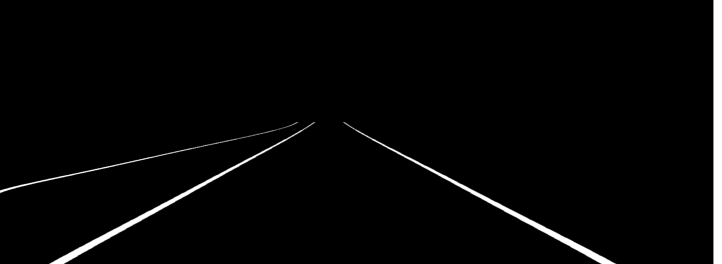
\includegraphics[width=\linewidth]{9.png}
  \caption{Binary Labels}
  \label{fig:labels2}
\end{figure}

\begin{figure}
  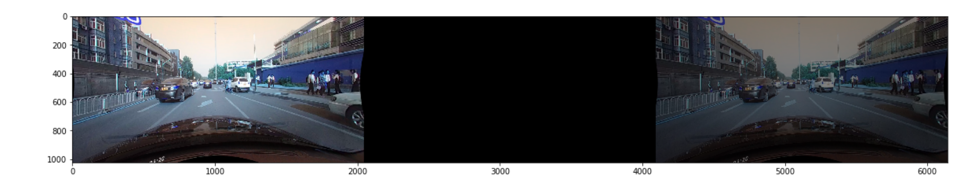
\includegraphics[width=\linewidth]{8.png}
  \caption{Image trained with binary labels.}
  \label{fig:badbad}
\end{figure}

\par The future steps to solve this problem would be to try to figure out exactly why is the model ignoring one of the labels and change how the model weights background pixels and label pixels, and make sure that the label pixels are weighted slightly more than the background.

%------------------------------------------------

\section{Conclusion}
At the beginning of the quarter, we set a few goals regarding this project. The very first steps were to combine the code from Lab 1 (Victoria) and then find out the speed and accuracy of that code to use as benchmark (Calvin). This gave us a basic structure to improve upon. We then explored different clustering alogrithms and replaced the window search with DBScan clustering technique (Daniel). Our next goals included benchmarking deep learning models, such as SCNN, LaneNet, and ICNet, however, we ran into difficulties running those models. We tried running SCNN and spent most of the time fixing ICNet to work as a lane line detection model (Victoria), and we also looked at the LaneNet model (Calvin). We were also planning on recording our own video and testing the lane line detection models we came up with on that video, but unfortunately we ran into some set backs along the way and did not accomplish this goal.

%----------------------------------------------------------------------------------------

\end{document}
